%%%%%%%%%%%%%%%%%%%%%%%%%%%%%%%%%%%%%%%%%%%%%%%%%%%%%%%%%%%%%%%%%%%%%%
% LaTeX Example: Project Report
%
% Source: http://www.howtotex.com
%
% Feel free to distribute this example, but please keep the referral
% to howtotex.com
% Date: March 2011 
% 
%%%%%%%%%%%%%%%%%%%%%%%%%%%%%%%%%%%%%%%%%%%%%%%%%%%%%%%%%%%%%%%%%%%%%%
% How to use writeLaTeX: 
%
% You edit the source code here on the left, and the preview on the
% right shows you the result within a few seconds.
%
% Bookmark this page and share the URL with your co-authors. They can
% edit at the same time!
%
% You can upload figures, bibliographies, custom classes and
% styles using the files menu.
%
% If you're new to LaTeX, the wikibook is a great place to start:
% http://en.wikibooks.org/wiki/LaTeX
%
%%%%%%%%%%%%%%%%%%%%%%%%%%%%%%%%%%%%%%%%%%%%%%%%%%%%%%%%%%%%%%%%%%%%%%
% Edit the title below to update the display in My Documents
%\title{Project Report}
%
%%% Preamble
\documentclass[paper=a4, fontsize=11pt]{scrartcl}
\usepackage[T1]{fontenc}
\usepackage{fourier}

\usepackage[english]{babel}															% English language/hyphenation
\usepackage[protrusion=true,expansion=true]{microtype}	
\usepackage{amsmath,amsfonts,amsthm} % Math packages
\usepackage[pdftex]{graphicx}	
\usepackage{url} 
\usepackage{caption}
\usepackage{subcaption}


\usepackage{listings}

%%% Custom sectioning
\usepackage{sectsty}
\allsectionsfont{\normalfont    }%\scshape\centering 


%%% Custom headers/footers (fancyhdr package)
\usepackage{fancyhdr}
\pagestyle{fancyplain}
\fancyhead{}											% No page header
\fancyfoot[L]{}											% Empty 
\fancyfoot[C]{}											% Empty
\fancyfoot[R]{\thepage}									% Pagenumbering
\renewcommand{\headrulewidth}{0pt}			% Remove header underlines
\renewcommand{\footrulewidth}{0pt}				% Remove footer underlines
\setlength{\headheight}{13.6pt}
\newcommand\tab[1][1cm]{\hspace*{#1}}

%%% Equation and float numbering
\numberwithin{equation}{section}		% Equationnumbering: section.eq#
\numberwithin{figure}{section}			% Figurenumbering: section.fig#
\numberwithin{table}{section}				% Tablenumbering: section.tab#


%%% Maketitle metadata
\newcommand{\horrule}[1]{\rule{\linewidth}{#1}} 	% Horizontal rule

\title{
	%\vspace{-1in} 	
	\usefont{OT1}{bch}{b}{n}
	\normalfont \normalsize \textsc{  Udacity Machine learning nanodegree - Project 4} \\ [25pt]
	\horrule{0.5pt} \\[0.4cm]
	\huge Train A Smartcab To Drive \\
	\horrule{2pt} \\[0.5cm]
}
\author{
	\normalfont 								\normalsize
	Sidharth Somanathan\\[-3pt]		\normalsize
	\today
}
\date{}


%%% Begin document
\begin{document}
	\maketitle 
	
	\section{Implement a Basic Driving Agent} 
	

In the code given to us a grid of roads is simulated which has a primary driving agent and few other cars. We have a grid of size 8 columns and 6 rows representing roads which intersect at 48 intersections. The boundaries are in fact circular, meaning if you take a right turn from intersection (1,8) you will reach (1,1) or if you go straight ahead from (1,8) you will reach (6,8). Given this condition the maximum distance between any two points is 7 steps ( Like traveling from (1,1) to (3,4)).
	
	\subsection{\textit{Observe what you see with the agent's behavior as it takes random actions. Does the \textbf{smartcab} eventually make it to the destination? Are there any other interesting observations to note?}} 
 
 For our basic driving agent we begin by implementing a primary agent which moves randomly. For this we set in the code  

\begin{lstlisting} 
  action = random.choice( [ None, 'forward', 'left', 'right' ] ) 
\end{lstlisting} 
     
 Since the motions of the primary agent ("red car") are now totally random at each intersection, it is expected that it will take longer number of steps to reach the destination. So here we increase the hard deadline to 1000 and also the initial deadline is now just set to 0 instead of five times the distance between random 'start' and 'destination'.  So the changes in environment class are
 

\begin{lstlisting}        
  e.set_primary_agent(a, enforce_deadline=False) 
  hard_time_limit = -1000    #changed from 100	 
  deadline = 0     #changed from  'self.compute_dist(start,destination)*5'		
\end{lstlisting} 
 
 
 With this little tweak we run 1000 trials and find that our random agent always reaches the destination (in the worst case for the trials it took 693 steps to reach destination). On an average it takes 120 steps to reach the destination when the primary agent is moving totally randomly. This number may seem high but interestingly it is really skewed by the few outliers who took lot more steps to reach destination. In the histogram in Figure 1.1 we can see that majority of the trials finish under 100 steps. This is confirmed by the median number of steps for the 1000 trials, which is equal to 89.   
 
 \begin{figure}[!ht]
 	\caption{Histogram of Number of Steps taken to destination.}
 	\centering
 	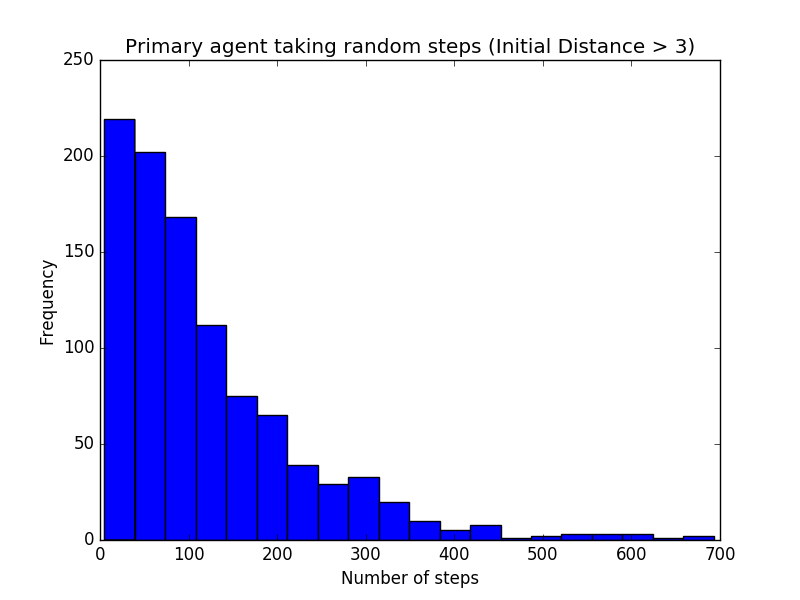
\includegraphics[width=0.7\textwidth]{hist3}
 \end{figure}
  
  
  Another interesting data to consider is that after 1000 trials we found the average net reward per trial was approximately -7.  This is quiet illuminating and the figure 1.2 sheds light on this, as we can see that in a individual trial it is possible to accumulate some positive reward points but mostly negative is the norm. This is represented by the blue dots. However the cumulative average (green dots) of all the trials prior and up to current one, relaxes to a negative value, which after 1000 trials turns out to be -6.9 in our case. This is to be expected since on an average when the primary agent is taking a random turn then it is more likely to get a negative reward.
  
  
  \begin{figure}[!ht]
  	\caption{Analysis plot of Net reward per trial and the average cumulative reward.}
  	\centering
  	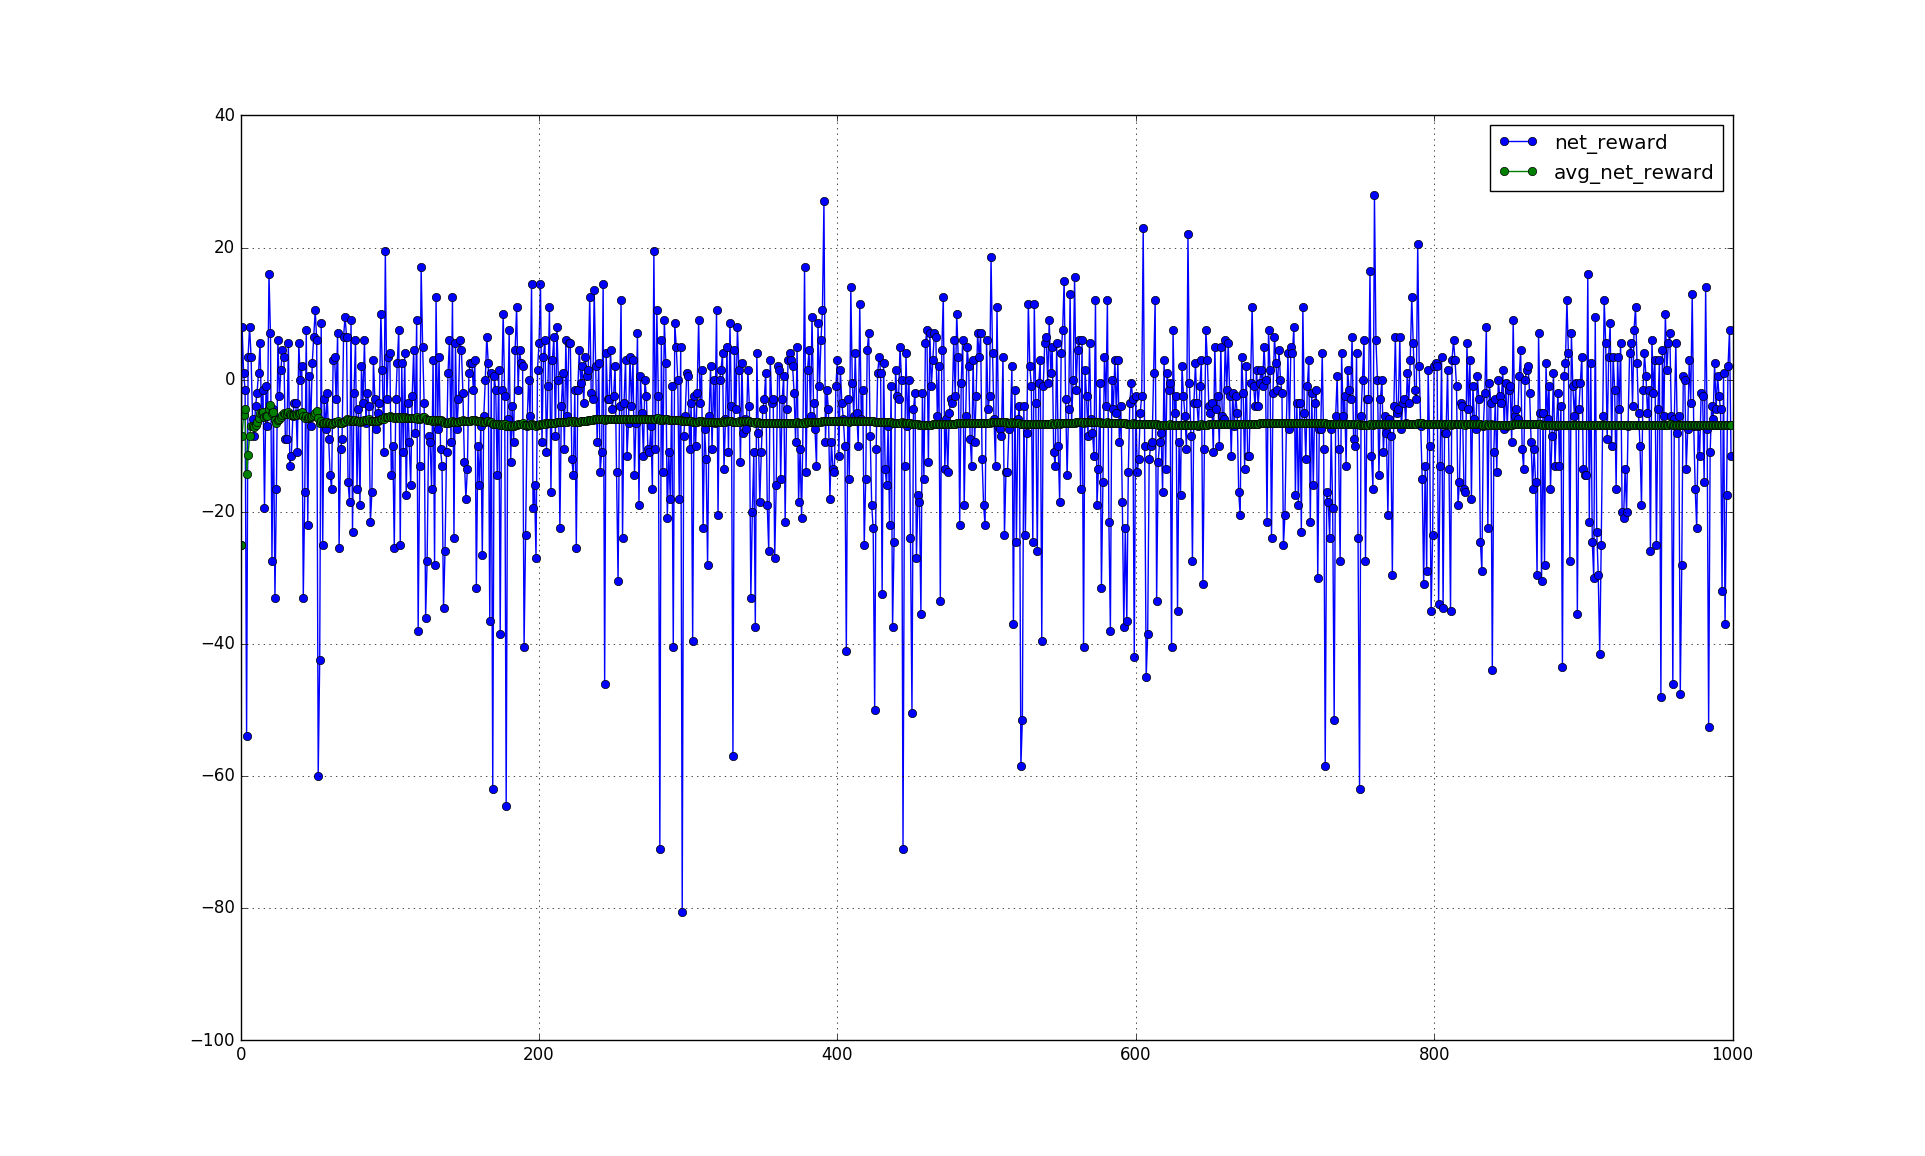
\includegraphics[width=0.7\textwidth]{avg-net-reward}
  \end{figure}
  
\pagebreak
\section{Inform the Driving Agent} 

\subsection{ \textit{What states have you identified that are appropriate for modeling the \textbf{smartcab} and environment? Why do you believe each of these states to be appropriate for this problem?} } 

Now as we want to improve on this random agent let us identify the states which would help us in model a \textit{smart} smartcab.  My choice of states are

\begin{itemize}
	\item   \texttt{self.next\_waypoint: } The next\_waypoint points towards the destination. Since this is like a compass and a signal towards our final aim, so this is something we certainly need as a state.
	\item   \texttt{self.inputs[\textquotesingle light\textquotesingle]: } The state of traffic light (red/green) is also essential as we want the smartcab to not violate traffic rules.
	\item   \texttt{self.inputs[\textquotesingle oncoming\textquotesingle]: } Even if the smartcab learns to move with green light and not move with green light, it still has to be mindful of the oncoming traffic from the front. Hence we use the state of the oncoming car if any.
	\item   \texttt{self.inputs[\textquotesingle left\textquotesingle ]: }  Same argument as last one for using the state of the car on the left.
\end{itemize}


The actions the smartcab has to take based on these states is either turn left, turn right, go forward or stay as it is (for red light or to follow traffic rules). Here we have ignored few other possible state like  \texttt{deadline} , \texttt{inputs[\textquotesingle right\textquotesingle]}. The problem with \texttt{deadline} as a state input is that this could make the state space very huge, which will slow down the program drastically. Values like  \texttt{deadline} can take values from 0 to around 30, which means it will increase state space from 96 (calculation of 96 in next section) to 96*30 approximately 3000. 
Similarly the state of the car to right can matter to the way the primary agent has to move. But since the car to the primary agents right can only move if the traffic light is red or if there is no traffic coming from left going to right. Both these cases are already being dealt by our existing choice of states (\texttt{self.inputs[\textquotesingle light\textquotesingle] },   \texttt{self.inputs[\textquotesingle left\textquotesingle ] }   ), and hence involving the state of  car to the right is superfluous.


\subsection{\textit{How many states in total exist for the \textbf{smartcab} in this environment? Does this number seem reasonable given that the goal of Q-Learning is to learn and make informed decisions about each state? Why or why not?}}

	Let us look at number of possible sub-states for each of the four major states we picked.
\begin{itemize}
	\item   \texttt{self.next\_waypoint: } 3  (forward, left or right).. notice none is not a possibility here.
	\item   \texttt{self.inputs[\textquotesingle light\textquotesingle]: } 2 (red or green)
	\item   \texttt{self.inputs[\textquotesingle oncoming\textquotesingle]: } 4 (The oncoming car could move right, left, forward or not move.)
	\item   \texttt{self.inputs[\textquotesingle left\textquotesingle ]: }  4 (The car on the left could move right, left, forward or not move.)
\end{itemize}


Hence in total we have 96 = ( 3*2*4*4) states. I think the number of states is more than sufficient for Q-Learning. Let's remember that we essentially have only three things to learn:- obey traffic lights, not collide with other vehicles by obeying  right of way at intersections and lastly to head towards destination. The 96 states covers all possible important combination of information needed to take an informed decision at an intersection. In fact with our simulation of 1000 trials and three dummy agents, we find that only 40 something of the 96 possible states are actually encountered as the algorithm quickly learns to reach the destination. However if we want the algorithm to learn over all the possible states then we really need lot more dummy agent traffic so that all possible situations are encountered. For instance when 100 dummy agents were initialized then all the 96 states were encountered at least once within 200 trials by the learning algorithm.
 
 \pagebreak
\section{Implement a Q-Learning Driving Agent}

\subsection{ \textit{What changes do you notice in the agent's behavior when compared to the basic driving agent when random actions were always taken? Why is this behavior occurring?}}

In Q-Learning algorithm we maintain a set of values for each state action pair. Whenever a state is encountered in the simulation the Q value is modified based on the following equation.
	\begin{align}\nonumber
	Q (s_t,a_t) =  (1  - \alpha)  \bigg[Q(s_t, a_t)  \bigg]+  \alpha \; \bigg[ r_{t+1}(s,a) + \gamma   \; \;  \max \; Q(s_{t+1}, a )   \bigg]
	\end{align}
	
Here $\alpha$ is the learning rate, $\alpha = 1$ means it will learn faster and accept more feedback from the update and $\alpha =0$ means it will ignore the feedback and keep the same Q-value. Similarly discount factor $\gamma$ is a measure of how much importance is to be given to the future reward/action.  Based on these updates, for each possible state-action pair, we will have a Q-value and the future action chosen for a given current state is the action with the maximum Q value. Hence when we let the simulation run long enough, the Q values keep getting modified to an apt value such that the algorithms learns what is the best possible action to be taken when the agent is in a given state.

After implementing the Q-Learning algorithm we find that the primary agent reaches must faster to the destination and in due course we see that the rate of negative reward gained per step is much less. In order to observe Q-Learning in action we run the simulation with 150 trials, with $\alpha=0.1$, $\gamma=0.5$. In Fig 3.1 we can see the total negative reward per trial drastically coming down as the agent learns policies to avoid incurring negative rewards. 

\begin{figure}
	\centering
	\begin{subfigure}{.6\textwidth}
		\centering
		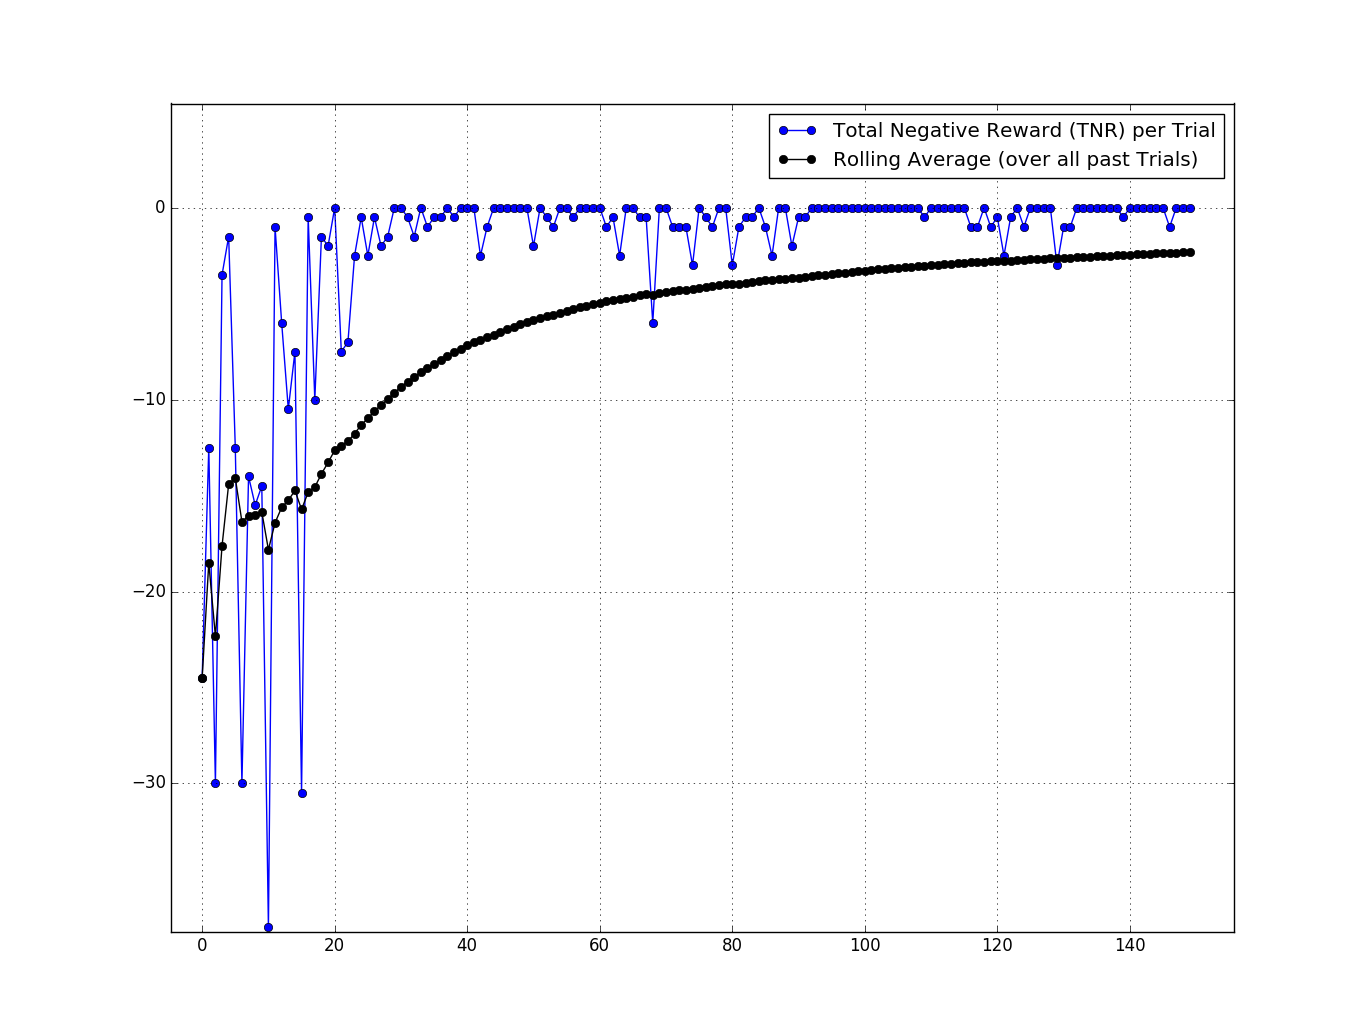
\includegraphics[width= \linewidth]{3_TNR}
		\caption{Plot of total negative reward   vs trial number.}
		\label{fig:sub1}
	\end{subfigure}%
	\begin{subfigure}{.56\textwidth}
		\centering
		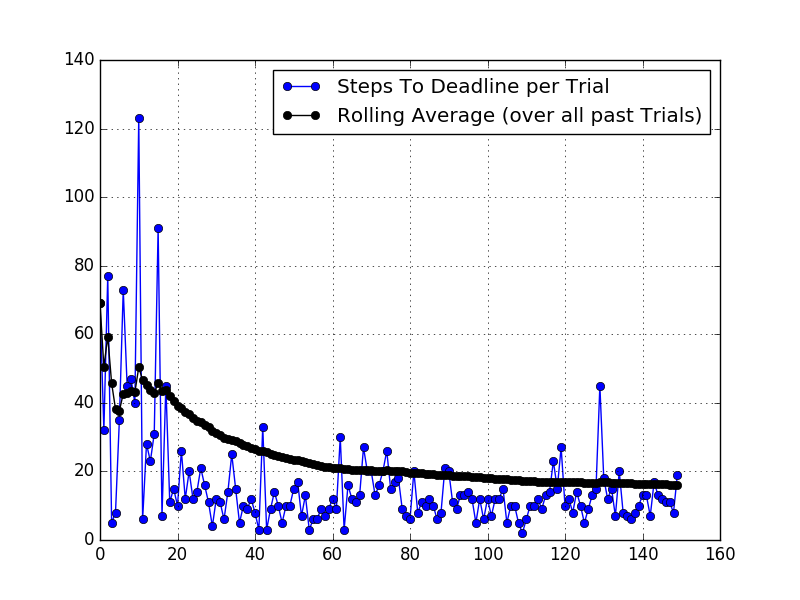
\includegraphics[width= \linewidth]{3_STD}
		\caption{Plot of steps taken to destination vs trial number.}
		\label{fig:sub2}
	\end{subfigure}
	\caption{A simulation of 150 trials with Q-Learning algorithm.   }
	\label{fig:test}
\end{figure}


\pagebreak
\section{Improve the Q-Learning Driving Agent}
\subsection{ \textit{Report the different values for the parameters tuned in your basic implementation of Q-Learning. For which set of parameters does the agent perform best? How well does the final driving agent perform?}}
 
 One of the enhancement I did was initally I had the state of the cab to the 'right' as one of the input state. I found it to be of no consequence to the speed of learning and was increasing the state space size and decreasing the speed of program. So I got rid of it and rest of the simulation were done without this state. 
 
 Since we start with Q-Values initialized to $15$ for all state action pairs, it is a good idea to start with a faster learning rate and not give much importance to the existence value. In Fig 3.1 we had showed the results with learning rate $\alpha =0.1$. Here in Fig 4.1 we show the results with a higher learning rate $\alpha=0.9$, lower discount rate $\gamma =0.2$, (giving importance to faster learning and immediate rewards). Please notice how fast the negative rewards are heading to zero per trial and we also converge to the optimal number of steps to destination also faster. Another interesting thing to notice in Fig 4.1(b) is that by end of 150 trials the average steps to destination was only 13.5. To really appreciate the Q-learning algorithm compare these plots with Figure 1.1 and Figure 1.2 where a random agent took more than 100 steps on average to reach destination and the net reward hovered randomly between positive and negative values.
 
 
 
 \begin{figure}
 	\centering
 	\begin{subfigure}{.6\textwidth}
 		\centering
 		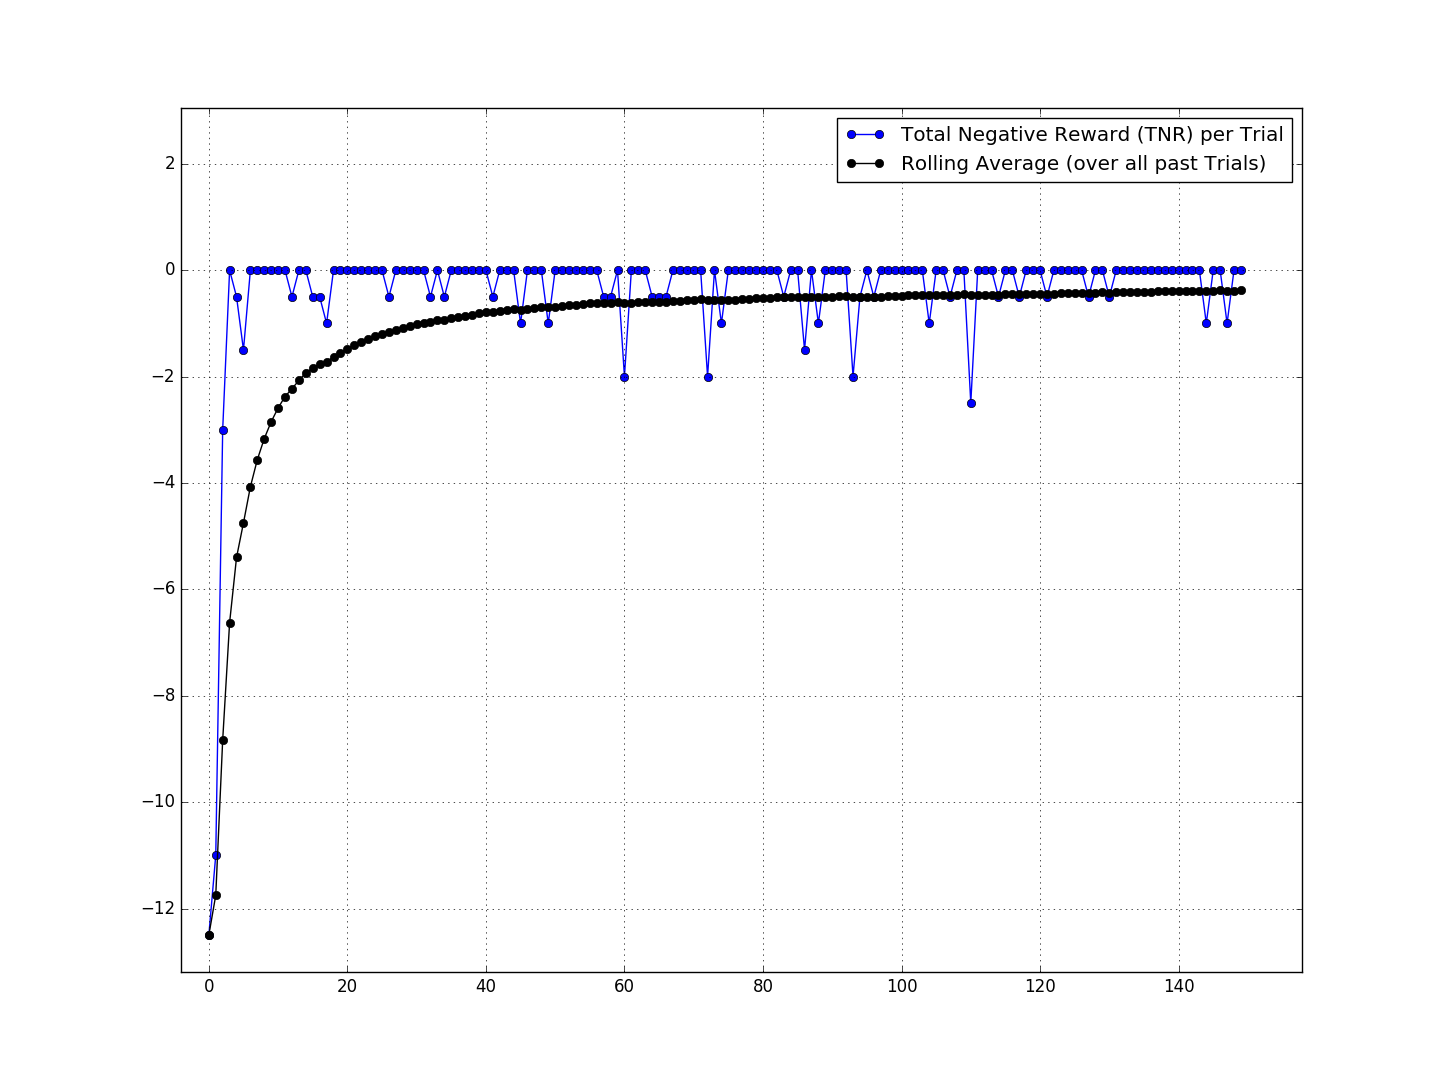
\includegraphics[width= \linewidth]{4_TNR}
 		\caption{Plot of total negative reward   vs trial number.}
 		\label{fig:sub1}
 	\end{subfigure}%
 	\begin{subfigure}{.6\textwidth}
 		\centering
 		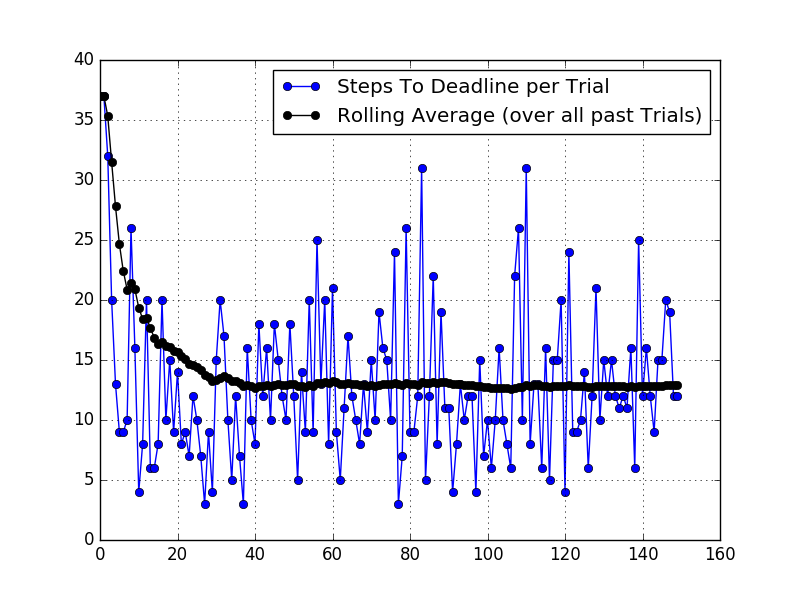
\includegraphics[width= \linewidth]{4_STD}
 		\caption{Plot of steps taken to destination vs trial number.}
 		\label{fig:sub2}
 	\end{subfigure}
 	\caption{A simulation of 150 trials with Q-Learning algorithm.   }
 	\label{fig:test}
 \end{figure} 
 
 \pagebreak
\section{CASE: What can a learned/trained agent do?}



\subsection{\textit{Does your agent get close to finding an optimal policy, i.e. reach the destination in the minimum possible time, and not incur any penalties? How would you describe an optimal policy for this problem?}}


In order to see how well Q-Learning can do, we ran the simulation for 100000 trial with 20 dummy cars in the simulation. This can be done in less than 10 minutes if we turn off display and reduce \texttt{update\_display} to a very small value. What this does is that the simulation goes into each of the 96 states enough times so that the Q-Table has updated and "learned" values after 10000 trials for every state-action pair. At the end of simulation we save the Q-values for each state action pair in a pickle file. This set of learned Q values were then used to run a 200 trials with 3 dummy cars. Interestingly we find that in each of the 200 trials not a single time the primary agent earns a negative rewards, this can be seen in Fig 5.1(a). And in Fig 5.1(b) we see the steps taken to destination per trial plot. The blue dots as expected hover around a little randomly, this is expected because we have three dummy cars roaming around randomly. So in each trial the primary agent might encounter them at intersections and get delayed. But the interesting thing to notice is the relatively small number of steps to reach destination, for instance after these 200 trials the average steps to reach destination is only 11.6. Let's remember 'steps' not only mean actual turns taken by smartcab, but also not taking an action to avoid negative rewards (aka accidents/traffic violations).


\begin{figure}
	\centering
	\begin{subfigure}{.45\textwidth}
		\centering
		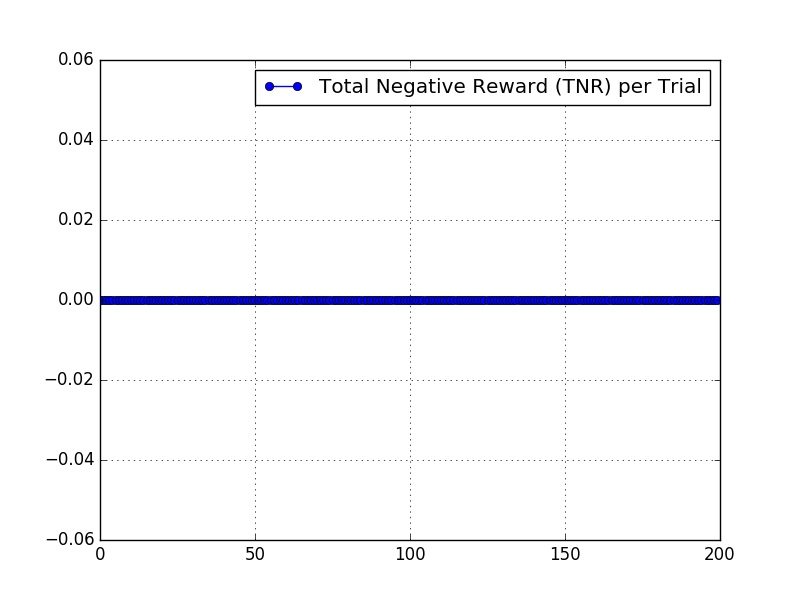
\includegraphics[width= \linewidth]{TNR_100000}
		\caption{Analysis plot of Total Negative Reward per trial, here simulation starts with the 100000 trial Q Learned values as initial Q values.}
		\label{fig:sub1}
	\end{subfigure}%
	\begin{subfigure}{.45\textwidth}
		\centering
		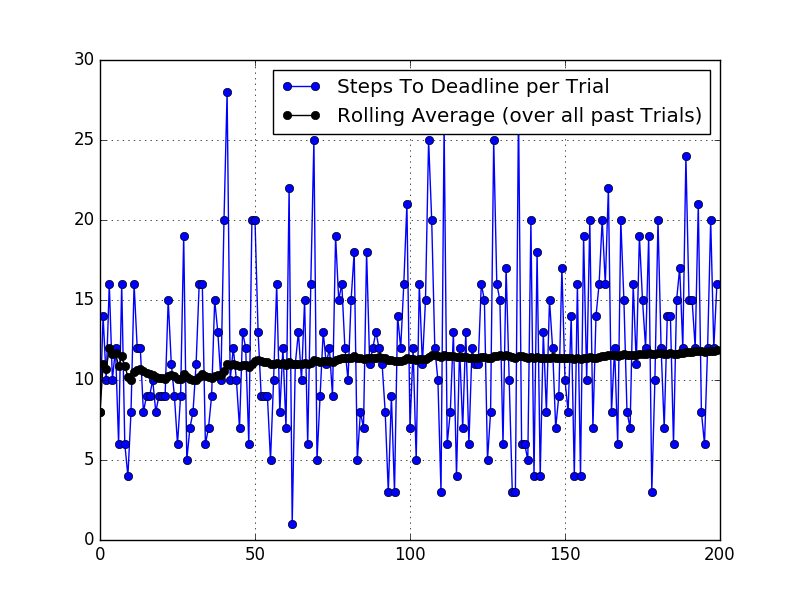
\includegraphics[width= \linewidth]{STD_100000}
		\caption{Analysis plot of Steps To Destination per trial, here simulation starts with the 100000 trial Q Learned values as initial Q values.}
		\label{fig:sub2}
	\end{subfigure}
	\caption{A simulation of 200 trials with a well trained Q-Learning model. }
	\label{fig:test}
\end{figure}


Here we can strongly conclude that after running 100000 trial simulation and updating the Q-table, we have discovered the optimal policy for this simulation. We expect this Q-table to show the best action for each of the 96 states. Let us take a look at a snippet of the dictionary (Q-Table) after 100000 trials. 

\texttt{ 
	\tab ('forward', 'green', None, None):\\
	\tab\tab	 \{\\
	\tab\tab\tab	None: 1.4375,\\
	\tab\tab\tab	'forward': 2.666668255425604,\\
	\tab\tab\tab	'left': 0.9375,\\
	\tab\tab\tab	'right': 1.375\\
	\tab\tab	 \},\\
	\tab ('forward', 'green', None, 'forward'):\\ 
	\tab\tab	\{\\
	\tab\tab\tab	None: 0.727294921875,\\
	\tab\tab\tab    'forward': 3.9598337809252184,\\
	\tab\tab\tab	'left': 1.53125,\\
	\tab\tab\tab	'right': 1.6875\},\\
	\tab\tab	\}\\	
	\tab\tab	.....\\
}

Here, for instance we can see that if the direction to destination is 'forward' (the waypoint), the traffic light is green, and there is no oncoming traffic or traffic to left, in that case the action with highest Q-value is 'Forward'. Hence the smartcab in  this state will continue to go forward, this is the optimal policy agent has learned for this state. 

After these 100000 trials we can safely say that the algorithm has learned 96 optimal policies and did not encounter any negative reward. This is evident from the 200 subsequent trials (Fig 5.1(a)) done with these learned policies. Also in Fig 5.1(b) we see the smartcab reached to destination with around 11.5 steps in average, which is a great gain compared to our random agent from Section 1.
 
 
 
	 
\begin{figure}
 	\centering
 	\begin{subfigure}{.5\textwidth}
 		\centering
 		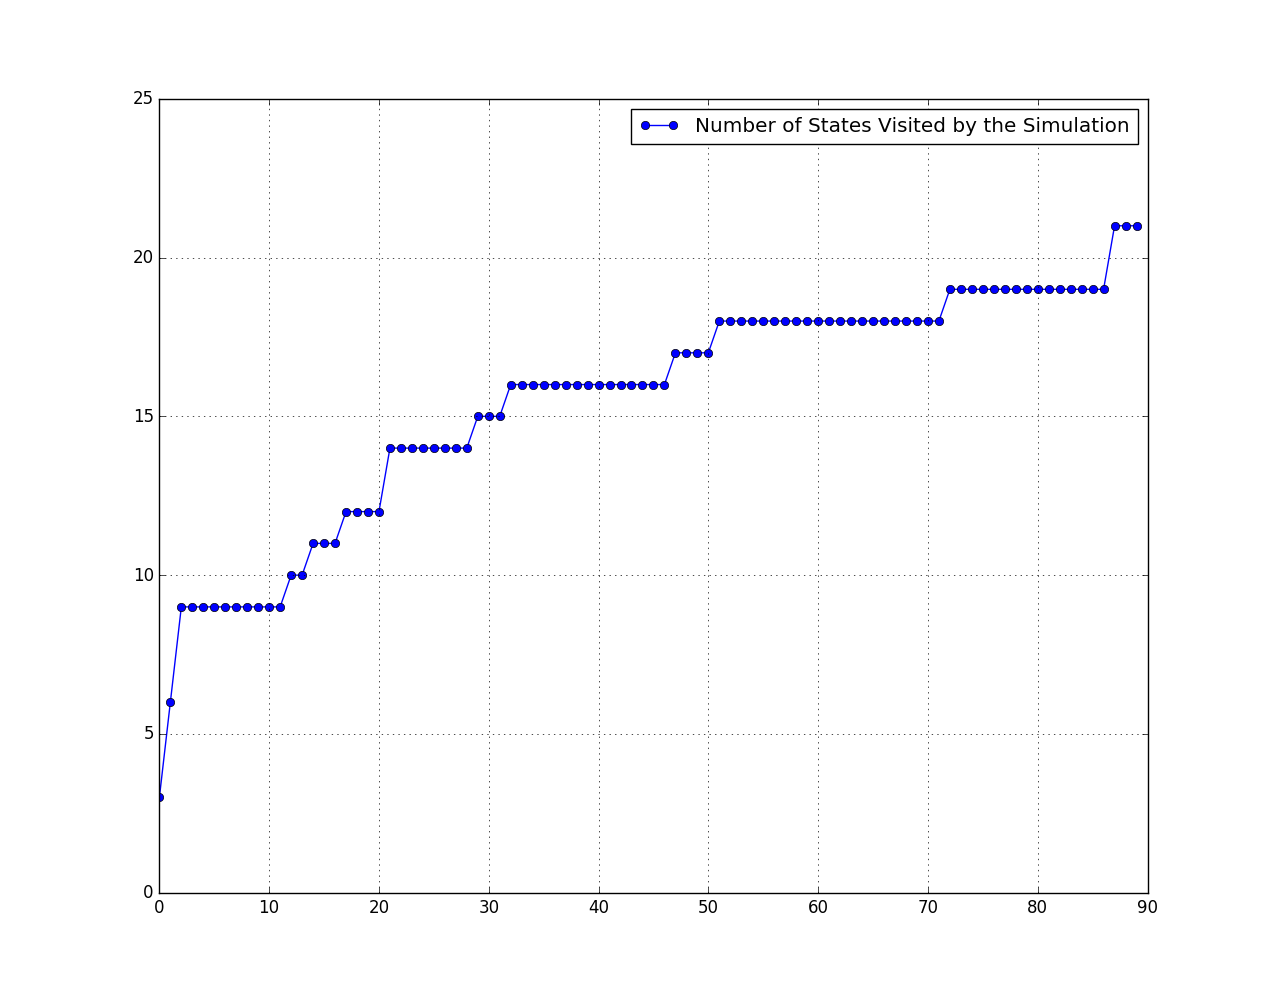
\includegraphics[width= \linewidth]{5_STATES}
 		\caption{Total number of states encountered.}
 		\label{fig:sub1}
 	\end{subfigure}%
 	\begin{subfigure}{.5\textwidth}
 		\centering
 		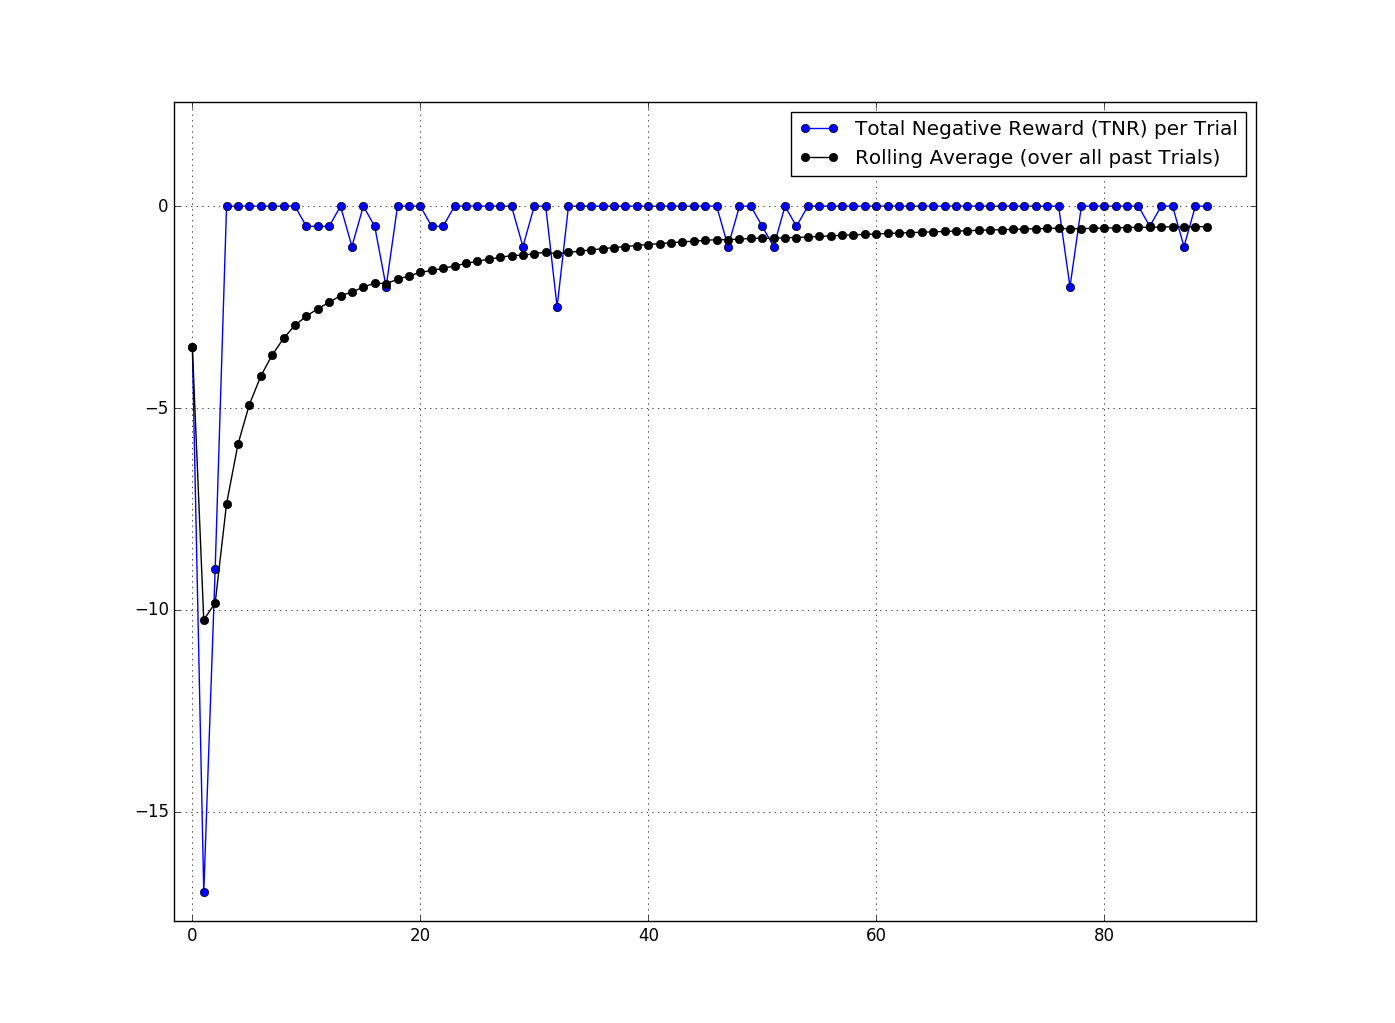
\includegraphics[width= \linewidth]{5_TNR}
 		\caption{Analysis plot of total negative reward per trial and its rolling average.}
 		\label{fig:sub2}
 	\end{subfigure}
 	\caption{A simulation of 90 training trials. }
 	\label{fig:test}
\end{figure}




\begin{figure}
	\centering
	\begin{subfigure}{.5\textwidth}
		\centering
		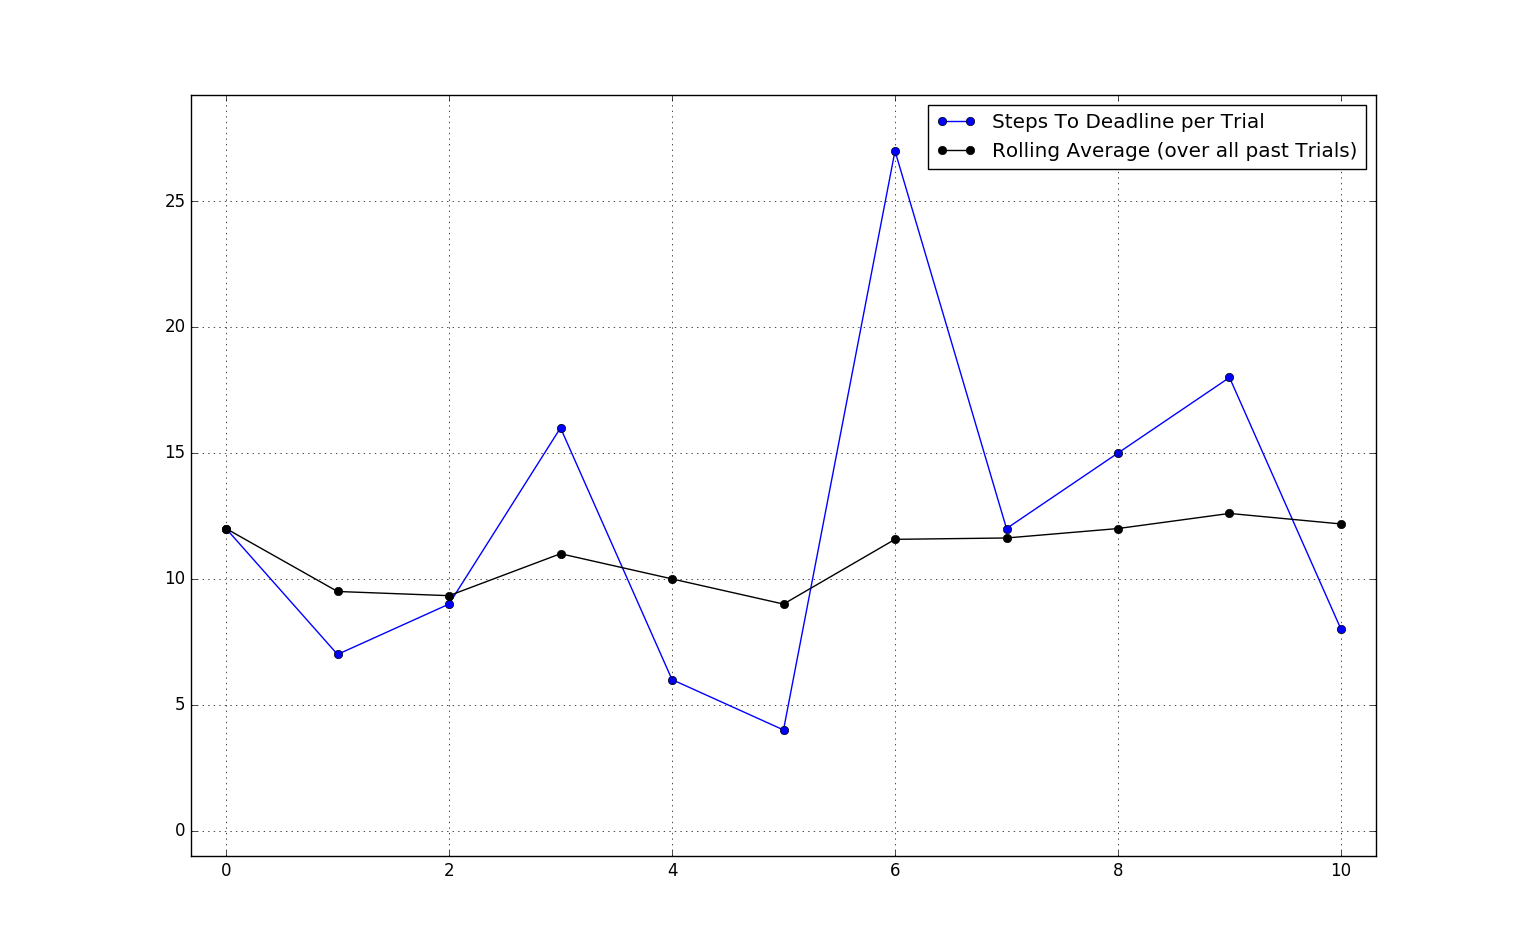
\includegraphics[width= \linewidth]{5_STEPS_10}
		\caption{Total number of steps to destination.}
		\label{fig:sub1}
	\end{subfigure}%
	\begin{subfigure}{.5\textwidth}
		\centering
		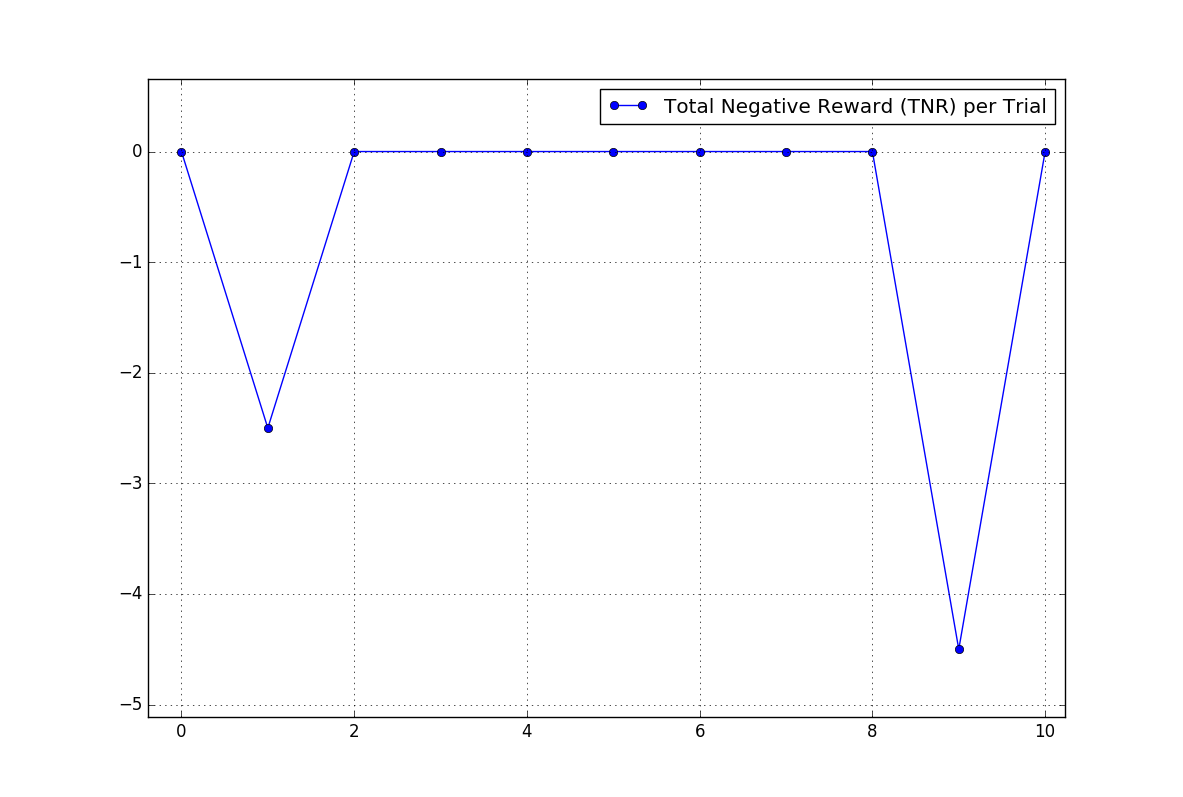
\includegraphics[width= \linewidth]{5_TNR_10}
		\caption{Analysis plot of total negative reward per trial and its rolling average.}
		\label{fig:sub2}
	\end{subfigure}
	\caption{A simulation of 10 evaluation trials using the learned model. }
	\label{fig:test}
\end{figure}

We can clearly see that agent learns well when 100000 trials were given. Now let us actually train it to the original constraints with 90 trials and then do a evaluation run with the learned Q-values for another 10 trials. The results from the training can be seen in Figure 5.2. One can notice that in these 90 trials the simulation encounters only encounters around 21 out of 96 possible states (Fig 5.2(a)), but even with around only quarter of states explored we can see that the total negative rewards has come down drastically (Fig 5.2(b))




Now let us see how this "90 trial" learned algorithm performs. We perform 10 evaluation trials with the previously trained model. In Figure 5.3(a) we can see that the average number of steps to destination is roughly 13 which is a descent for performance for a very shortly trained model.  More interestingly we find that net negative reward for the 10 trials remains zero, 8 times out of 10. Even the 2 times it goes negative, the number is not too large. So we can see that even this lightly trained Q-Learning model (with $\alpha = 0.9$, $\gamma = 0.2$ \& $90$ trials ) performs more than reasonably well.
	  
	  


\end{document}